\section{Execution}
\label{sec:execution}

This chapter explains how the experiment is set up and carried out.

\subsection{Set Up}
\label{sec:setup}

The set up follows \autoref{fig:rbsetup}. Breaking down the set up the laser already contains the collimating lens and the grating optics as can be seen in \autoref{fig:laser_setup}.
The elements of the laser head are arranged in such a way that they follow the Littrow-configuration. 
This means that the collimating lens in the laser head refracts the light in a way that the light rays run parallel to each other.
After the lens the grating refracts the first order maxima back into the laser chip and provides an optical feedback.
A screw on the laser head can be turned to rotate the grating, which changes the lasers wavelength. 
This also effects the direction of the output beam.
The next elements in the optical path is a polarization filter, that ensures the linear polarization of the beam.  

\begin{figure}[H]
    \centering
    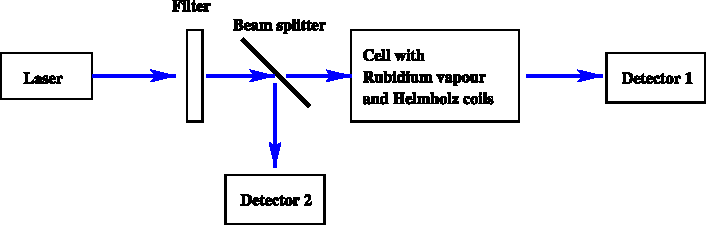
\includegraphics{figures/rbsetup.pdf}
    \caption{Diagram of the experimental set up \cite{v60}.}
    \label{fig:rbsetup}
\end{figure}

\begin{figure}[H]
    \centering
    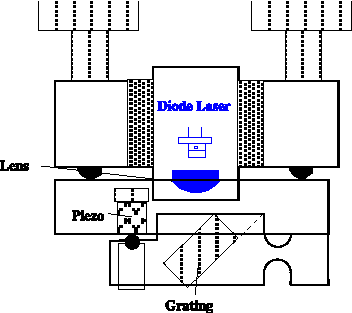
\includegraphics{figures/laser_setup.pdf}
    \caption{Diagram the laser head \cite{v60}.}
    \label{fig:laser_setup}
\end{figure}

\subsection{Threshold Current}
\label{sec:ThresholdCurrent}

This section describes the steps to measure the threshold current. 
The threshold current is the current that must be applied to the diode chip for lasing to occur.
Below this current no laser effects can be seen and the diode operates as an LED.
For this one can place an "IR Viewing Card" in the light beams path.
If the set up is actually lasing smaller "speckles" should appear in the vicinity of point where the main beam hits the card.
These speckles are the result of interference effects if laser light hits the surface of the card. 
Because the surface contains small irregularities, secondary light waves are created that can superimpose each other forming a distribution of these speckles on the surface of the card.\\
If no lasing takes place the light beam would only form one large point on card, because the secondary light waves are not coherent enough to interfere.\\

For this measurement the room light is dimmed, the IR Viewing Card is placed inside the beam and CCD-Camera focused on the card.
Now the current is slowly increased until the speckles are visible.

\subsection{Florescence and Absorption Spectrum of Rubidium}
\label{sec:Spectrum}

For this measurement the set up is arranged as depicted in \autoref{fig:rbsetup}.
To see florescence of rubidium the laser has to powerful enough.
For this the current has to significant higher than the threshold current.
Other ways to increase the strength of the laser is to improve the alignment by changing the angle of the grating or the current that flows throw the piezo cristall.
If the florescence can be seen a picture of the monitor that is hookup to CCD-Camera can be taken.\\

To measure to transmission spectrum the beam is splittet with a $50 \mathbin{/}50$ beam splitter.
One half is directly send to photo diode. 
The second half ist sent through a the rubidium cell and is than detected by a different photo diode.
To reduce background noise both photo diodes are connected to a function generator as input that gives the difference of both currents as an output to a oscilloscope.
It is necessary to align all components in a way that no mode hopping is visible, because this hopping would distort the spectrum. 